
\section{Dataset source}
The dataset used is gotten from \href{https://www.kaggle.com/datasets/fedesoriano/heart-failure-prediction}{kaggle} and was made by putting together different datasets that were already out there but had never been put together before. In this dataset, 5 heart datasets are put together based on 11 common features. This makes it the largest dataset for heart disease research that has been made available so far. The five datasets that were used to put it together are:
\begin{itemize}
	\item Cleveland: 303 observations
	\item Hungarian: 294 observations
	\item Switzerland: 123 observations
	\item Long Beach VA: 200 observations
	\item Stalog (Heart) Data Set: 270 observations
\end{itemize}

\comment{The classification process was carried out with the use of k-nn, naive bayes, decision tree, and logistic regression algorithms.}

\section{Exploratory data analysis}
\begin{figure}[htb]
	\centering
	\makebox[0cm]{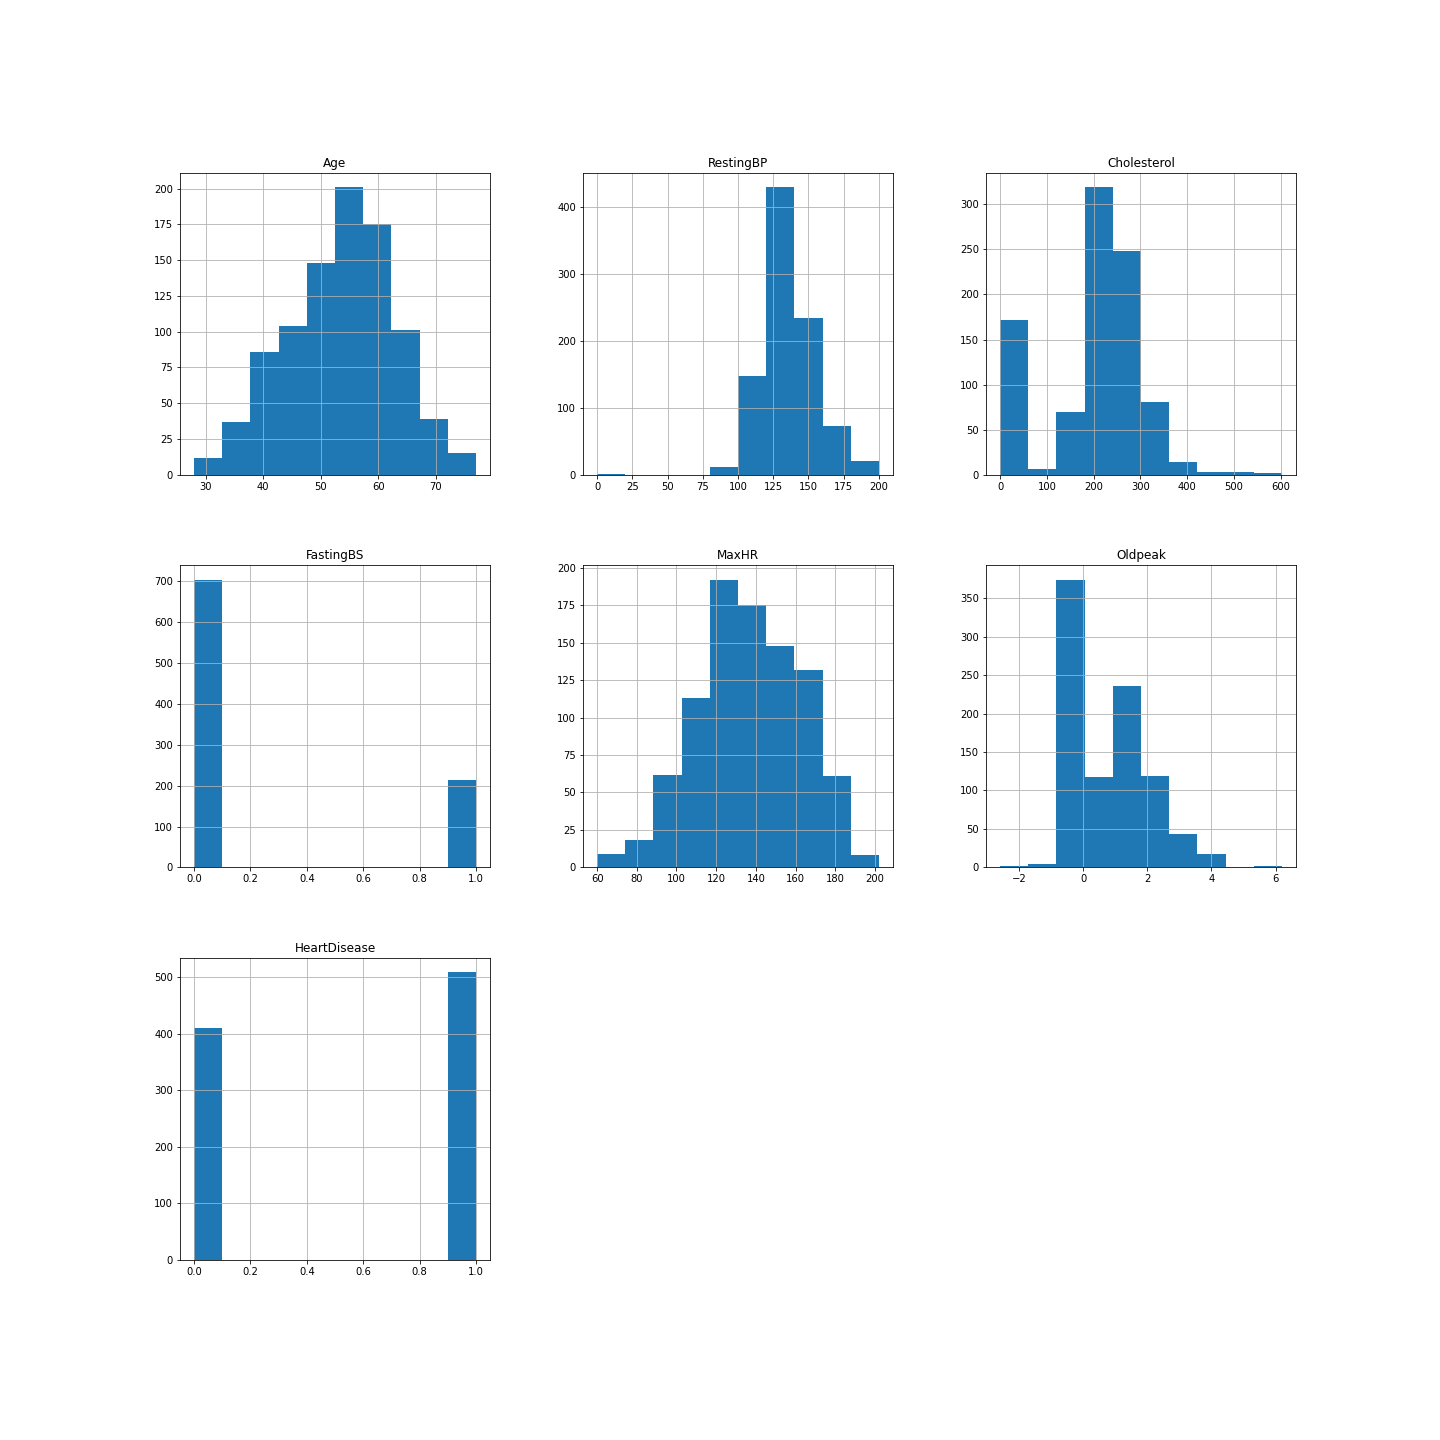
\includegraphics[scale=0.4]{df-histogram.png}}
	\caption{Histogram of numerical features in the dataset}
	\label{fig:df-histogram}
\end{figure}

\begin{figure}[htb]
	\centering
	\makebox[0cm]{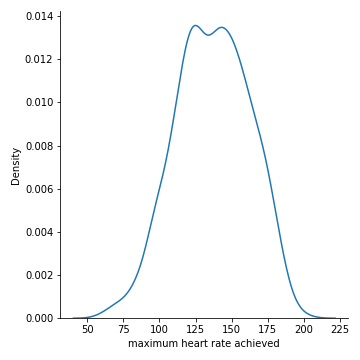
\includegraphics[scale=0.8]{max-heart-rate.png}}
	\caption{Maximum heart rate achieved}
	\label{fig:max-heart-rate}
\end{figure}

\section{Data preprocessing}
The preprocessing steps in the following subsections were applied on the dataset.
\subsection{Imputation}
Before imputation, we have to check for missing values in the dataset.
\begin{lstlisting}[language=Python, caption=Dataset information]
	df.info()\end{lstlisting}
Output:
\begin{lstlisting}[numbers=none]
	RangeIndex: 918 entries, 0 to 917
	Data columns (total 12 columns):
	#   Column          Non-Null Count  Dtype  
	---  ------          --------------  -----  
	0   Age             918 non-null    int64  
	1   Sex             918 non-null    object 
	2   ChestPainType   918 non-null    object 
	3   RestingBP       918 non-null    int64  
	4   Cholesterol     918 non-null    int64  
	5   FastingBS       918 non-null    int64  
	6   RestingECG      918 non-null    object 
	7   MaxHR           918 non-null    int64  
	8   ExerciseAngina  918 non-null    object 
	9   Oldpeak         918 non-null    float64
	10  ST_Slope        918 non-null    object 
	11  HeartDisease    918 non-null    int64  
	dtypes: float64(1), int64(6), object(5)
	memory usage: 86.2+ KB
\end{lstlisting}


We can see from the output that there are no null values in the dataset. Also, The \textit{string} columns in the dataset are represented as \textit{object} and need to be converted to \textit{string} types.


\begin{lstlisting}[language=Python, caption={Convert object columns to string}]
	string_col = df.select_dtypes(include="object").columns
	df[string_col]=df[string_col].astype("string")
\end{lstlisting}



\section{Testing}

\section{Performance analysis}